\documentclass[11pt]{article}
\usepackage[scaled=0.92]{helvet}
\usepackage{geometry}
\geometry{letterpaper,tmargin=1in,bmargin=1in,lmargin=1in,rmargin=1in}
\usepackage[parfill]{parskip} % Activate to begin paragraphs with an empty line rather than an indent %\usepackage{graphicx}
\usepackage{amsmath,amssymb, mathrsfs, dsfont}
\usepackage{tabularx}
\usepackage[font=footnotesize,labelfont=bf]{caption}
\usepackage{graphicx}
\usepackage{xcolor}
%\usepackage[linkbordercolor ={1 1 1} ]{hyperref}
%\usepackage[sf]{titlesec}
\usepackage{natbib}
\usepackage{../../Tianpei_Report}

%\usepackage{appendix}
%\usepackage{algorithm}
%\usepackage{algorithmic}

%\renewcommand{\algorithmicrequire}{\textbf{Input:}}
%\renewcommand{\algorithmicensure}{\textbf{Output:}}



\begin{document}
\title{Lecture 1: Introduction to Reinforcement Learning}
\author{ Tianpei Xie}
\date{ Dec 27th., 2017 }
\maketitle
\tableofcontents
\newpage
\section{Reinforcement Learning}
The study of machine learning can be divided into three categories:
\begin{enumerate}
\item \textbf{Supervised learning}.  \underline{Learning to \emph{\textbf{predict}} and \emph{\textbf{generalize}}}. In other words, the task of learning is to infer a mapping between covariates (data) and responses (target) so that the error/cost is minimized. Each example is a description of situation (sample) together with a specification (label) of the correct action the system should take to that action. Supervised learning is an \textbf{error-correction} process. It is an one-step prediction. Human label is used as  \underline{\textbf{instructive feedbacks}}. 

\item \textbf{Unsupervised learning}.  \underline{Learning to \emph{represent} and \emph{discover} the  hidden structure of data}. A proper representation of data facilitates knowledge discovery and improves the performance of prediction. It also helps in visualization, storage and communication. 

\item \textbf{Reinforcement learning}. \underline{Learning from \emph{\textbf{interaction}}}. As compared to above approaches,  reinforcement learning studies \underline{\emph{goal-directed}} \emph{learning from interaction}. The term 'learning' means learning to map \emph{situations} to  \underline{\emph{actions}} so as to maximize the reward. Also it is often unrealistic to obtain all examples of desired behavior that are both correct and representative of all situations in which the agents have to act. Reinforcement learning is a \textbf{trial-and-error} process and it is a multi-step prediction. It cares about future rewards in multiple steps. On the other hand, reinforcement learning only optimize the future rewards, where the rewards are used as  \underline{\textbf{evaluative feedbacks}}.  
\end{enumerate}

In reinforcement learning, the learner is not told which actions to take, but instead must discover which actions yield the most reward by \emph{trying} them. In the most interesting and challenging cases, actions may affect not only the immediate reward but also the next situation and, through that, all subsequent rewards. These two characteristics -- \textbf{trial-and-error search} and \textbf{delayed reward} -- are the two most important distinguishing features of reinforcement learning. Supervised learning algorthim enforces each step to be as instructed whereas the reinforcement learning agent only cares if the end goal is reached, and does not care the process. In supervised learning, we care about the \underline{\textbf{target}} predicted by the optimized learning model. In reinforcement learning, we care about the \underline{\textbf{process}} of getting it. RL is not to be confused with \underline{\textbf{\emph{online learning}}} \citep{cesa2006prediction, shalev2012online}, a method of machine learning in which data becomes available in a \emph{sequential} order and is used to update the best predictor for future data at each step. Both supervised learning and RL method can be online learning.

 
The basic theory behind reinforcement learning is dynamic systems theory, specifically, the optimal control of partially-known Markov decision processes. The idea is to capture the most important aspects of the real problem facing a \emph{learning agent} interacting over time with its \emph{environmen}t to achieve a goal. 

One of the challenges that arise in reinforcement learning, and not in other kinds of learning, is the \emph{trade-off} between  \underline{\emph{\textbf{exploration}} and \emph{\textbf{exploitation}}}. To obtain a lot of reward, a reinforcement learning agent must prefer actions that it has tried in the past and found to be effective in producing reward. But to discover such actions, it has to try actions that it has not selected before. The agent has to  \underline{\emph{exploit}} what it has \underline{already experienced in order to obtain reward}, but it also has to \underline{\emph{explore}} in order to make better action selections \underline{in the future}. The dilemma is that neither exploration nor exploitation can be pursued exclusively without failing at the task. The agent must try a variety of actions and \emph{progressively} favor those that appear to be best. On a stochastic task, each action must be tried many times to gain a reliable estimate of its expected reward. The \textbf{exploration-exploitation dilemma} has been intensively studied by mathematicians for many decades, yet remains unresolved.
\begin{itemize}
\item \textbf{exploitation}: the agent maximizes the rewards based on past experience

\item \textbf{exploration}: the agent interacts with environments for better actions in future
\end{itemize}


Another key feature of reinforcement learning is that it explicitly considers the \emph{whole} problem of a goal-directed agent interacting with an uncertain environment. It not only considers the learning sub-problem but also how it fits into a larger picture of decision making and \emph{planning}. A reinforcement learning agent is a complete, \underline{\emph{model-interactive}, \emph{goal-seeking}} object and usually operates facing significant uncertainties about the environment. When reinforcement learning involves planning, it has to address the interplay between planning and real-time action selection, as well as the question of how environment models are acquired and improved. When reinforcement learning involves supervised learning, it does so for specific reasons that determine which capabilities are critical and which are not. 

Terminologies in reinforcement learning:
\begin{itemize}
\item \textbf{Agent}: an object that is able to \emph{sense} the state of its environment to some extent and must be able to \emph{take actions} that \emph{affect} the state. The agent also must have a goal or goals relating to the state of the environment.

\item \textbf{Environment}: the surrounding field of the agent that is related to the problem to be solved. Environment also provides feedback regarding actions of an agent and defines the goal of the agents. The situation/information of environment that is sensible to the agent is referred as \emph{state} of environment. As it interacts with agents, the state of environment changes. 

\item \textbf{Policy}: defines the learning agent's way of behaving at a given time. Roughly speaking, a policy is a mapping from \emph{perceived states} of the environment to \emph{actions} to be taken when in those states. In some cases the policy may be a simple function or lookup table, whereas in others it may involve extensive computation such as a search process. The policy is the \emph{\textbf{core}} of a reinforcement learning agent in the sense that it alone is sufficient to determine behavior. In general, policies may be stochastic.

\item A \emph{\textbf{reward} signal} defines the goal in a reinforcement learning problem. On each time step, the environment sends to the reinforcement learning agent a single number called the \emph{reward}. The agent's sole objective is to maximize the \emph{\textbf{total reward}} it receives \emph{\textbf{over the long run}}. The reward signal thus defines what are the good and bad events for the agent. The reward signal is the primary basis for altering the policy; if an action selected by the policy is followed by low reward, then the policy may be changed to select some other action in that situation in the future. In general, reward signals may be \emph{stochastic} functions of the state of the environment and the actions taken.

\item \textbf{Returns} at $t$ is the cumulative rewards starting at time $t$. Return is the measure of rewards in long run. 

\item \emph{\textbf{Value function}}: specifies what is good  \underline{\emph{\textbf{in the long run}}}, whereas the reward signal specifies what is good in an  \underline{\emph{\textbf{immediate}}} sense. Roughly speaking, the value of a state is the total amount of reward an  agent can expect to accumulate over the future, starting from that state.

Rewards are in a sense \textbf{primary}, whereas  \underline{values, as predictions of rewards}, are \textbf{secondary}. Without rewards there could be no values, and the only purpose of estimating values is to achieve more reward. Nevertheless,  \underline{s \emph{values} with which we are most concerned} when making and evaluating decisions. Action choices are made based on \emph{value judgments}. The optimal actions should bring about states of highest values, not highest reward. Unfortunately, it is much harder to determine values than it is to determine rewards. Rewards are basically given directly by the environment, but values must be estimated and re-estimated from the sequences of observations an agent makes over its entire lifetime. The \emph{central role} of \emph{\textbf{value estimation}} is arguably the most important thing we have learned about reinforcement learning over the last few decades.

\item \emph{\textbf{Model}}: describes and mimics the behavior of the environment, or more generally, that allows inferences to be made about how the environment will behave. For example, given a state and action, the model might predict the resultant next state and next reward. Models are used for \emph{planning}, by which we mean any way of deciding on a course of action by considering possible future situations before they are actually experienced.

Methods for solving reinforcement learning problems that use models and \emph{planning} are called \emph{\textbf{model-based}} methods, as opposed to simpler \emph{\textbf{model-free}} methods that are explicitly \emph{trial-and-error} learners -- viewed as almost the \emph{opposite} of planning.

\item \emph{\textbf{exploration-exploitation tradeoff}}: the fundamental tradeoff for all reinforcement learning algorithms. Both exploration and exploitation require the agent to spend time and resources, while fail to balance them will result in agent's poor learning performance.
\begin{itemize}
\item \emph{\textbf{exploitation}}: the agent need to \emph{\textbf{optimize}} its policy and evaluation estimation performance based on accumulated experience by far. 

\item \emph{\textbf{exploration}}: the agent need to  \emph{\textbf{explore}} new actions and visit previously unvisited states in order to acquire new experience and search potential better policy, even if choosing these actions are not based on an optimal policy.
\end{itemize} The agent's goal is to exploit but without exploration it cannot gain enough feedbacks and experience about the environment, which would cause the agent to stuck in its \textbf{comfort zoon}. On the other hand, pure exploration without exploitation would cause the agent to not learn anything. 
\end{itemize}

There are approaches that do not belong to reinforcement learning. For instances, various \emph{evolutionary methods} including genetic algorithms and genetic programming, simulated annealing and other optimization methods have been used to search optimal policy without appealing to value functions. If the \emph{space of policies is sufficiently small}, or can be structured so that good policies are common or easy to find -- or if a lot of time is \emph{available for the search} -- then evolutionary methods can be effective.  In addition, evolutionary methods have advantages on problems in which the learning agent \emph{cannot sense the complete state} of its environment. On the other hand,  evolutionary methods do not interact with the environment but to evaluate the 'life-time' behavior of many non-learning agents.  Without the details of individual behavioral interactions, evolutionary methods ignores many useful structures that benefits the reinforcement learning.   Evolutionary methods also do not use the fact that the policy they are searching for is a function from states to actions; they do not notice which states an individual passes through during its lifetime, or which actions it selects. 

\section{Summary of methods learned}
We summarize our learning in the book \citep{sutton2018reinforcement}. Please comes back after finishing learning the main materials. 
\begin{figure}
\begin{minipage}[t]{1\linewidth}
  \centering
  \centerline{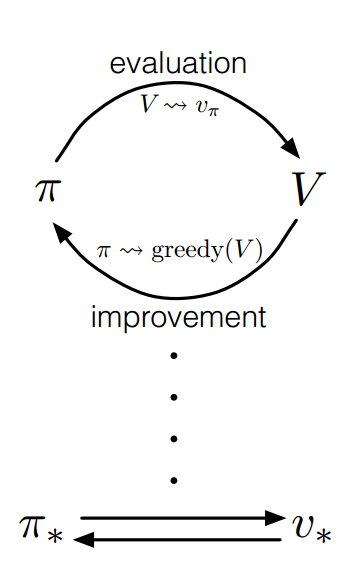
\includegraphics[scale = 0.3]{GPI.png}}
\end{minipage}
\caption{\footnotesize{\textbf{Generalized Policy iteration}}}
\label{fig: GPI}
\end{figure}
\subsection{From Multi-armed Bandit  to MDP}
The reinforcement learning methods we are discussing are based on Markov Decision Process. Simpler than MDP, we have the Multi-armed Bandit problem.
\begin{itemize}
\item \textbf{Multi-Armed Bandit problem (MAB)} (\emph{lecture 2}): in the classical Multi-armed bandit problem, there is only one state or it is \textbf{stationary}. Therefore, we \textbf{only care about the \emph{short-term gain}}, i.e. the rewards.  The goal is to select the action $a \in \set{1,\ldots, k}$ with highested \textbf{expected rewards}:
\begin{align*}
q_*(a) &:= \E{}{R_t \,|\, A_t = a}.
\end{align*} The solution for MAB is to compute the average of sample rewards. We use the incremental updates 
\begin{align}
Q_{n+1} &:= Q_{n} + \alpha_n(R_n - Q_n)\;\;\; \text{where }\alpha_n :=\frac{1}{n} \label{eqn: increment_update}\\
\Rightarrow \text{\textbf{new estimate}}&=\text{\textbf{old estimate}} + \text{stepsize}\,\cdot (\text{target} - \text{old estimate}) \nonumber
\end{align} The optimal action is selected via greedy or $\epsilon$-greedy algorithm based on the estimated expected reward for each action. 



\item  \textbf{The Markov Decision Process (MDP)} (\emph{lecture 3}): A MDP is a discrete-time stochastic control process. It is defined by the tuple \underline{$(T, \cS, \cA, \cR, P(S_{t+1}, R_{t+1} | S_{t}, A_{t}))$}, where $T$ defines the set of decison epochs,  $\cS$ is the state space,  $\cA$ is the action space, which is determined by the state selected, $\cR$ is the reward set. The conditional distribution $P(S_{t+1}, R_{t+1} | S_{t}, A_{t}))$ follows the \textbf{Markov property}, i.e.  the reward and next state is determined \textbf{completely} by its immediate predecessor state and action. $p(s', r| s, a)$ defines the dynamic of the process. $\pi: \cS \rightarrow \cA$ is the \emph{policy}, which is what we cared about the most. 

The process modeled by MDP is inherently dynamic and \textbf{non-stationary}. The objective of the agent is to find \emph{\textbf{optimal policy}} $\pi$ that \emph{maximizes} the  \textbf{long-term gain}, i.e. the cumulative future rewards,  or \textbf{expected returns}. To evalute the performance of a policy $\pi$, we introduce the value function 
\begin{align*}
v_{\pi}(s) &:= \E{\pi}{\sum_{\tau=0}^{T-t-1}\gamma^{\tau}R_{\tau+t+1} \Big|\, S_t = s};\\
q_{\pi}(s, a) &:= \E{\pi}{\sum_{\tau=0}^{T-t-1}\gamma^{\tau}R_{\tau+t+1} \Big|\, S_t = s, A_{t} = a}.
\end{align*} As we can see, the reinforcement learning based on MDP has two major steps:
\begin{itemize}
\item \textbf{Policy evaluation (Prediction)}: The task of policy evaluation is to \textbf{estimate} \emph{\textbf{value function}} $\hat{v}(s)$ and $\hat{q}(s, a)$ based on rewards collected in the sequence $(S_t, A_t, R_{t+1}, S_{t+1}, \ldots)$ as well as previous estimates (\textbf{boostrapping})

\item \textbf{Policy improvement (Control)}: The task of control is to find an \emph{\textbf{optimal policy}} $\pi_{*}$ given the value function from policy evaluation.
\end{itemize}The \textbf{generalized policy iteration (GPI)} (\emph{lecture 4}) defines an iterative procedure that loops between policy evaluation and policy improvement. Through this procedure, the agent is able to adapt and improve its policy by interactions with environment.  
\end{itemize} The theory of reinforcment learning overlaps with the \emph{\textbf{\underline{Stochastic Control} theory}} \citep{puterman2014markov} or \textbf{\emph{Optimal Control} theory}, where  \emph{action} is referred as \emph{control} and the \emph{environment} is the \emph{\textbf{dynamic system}} under control. The difference is that stochastic control theory focus more on model-based learning.

\subsection{Tabular methods vs. Function approximation}
\begin{figure}
\begin{minipage}[t]{1\linewidth}
  \centering
  \centerline{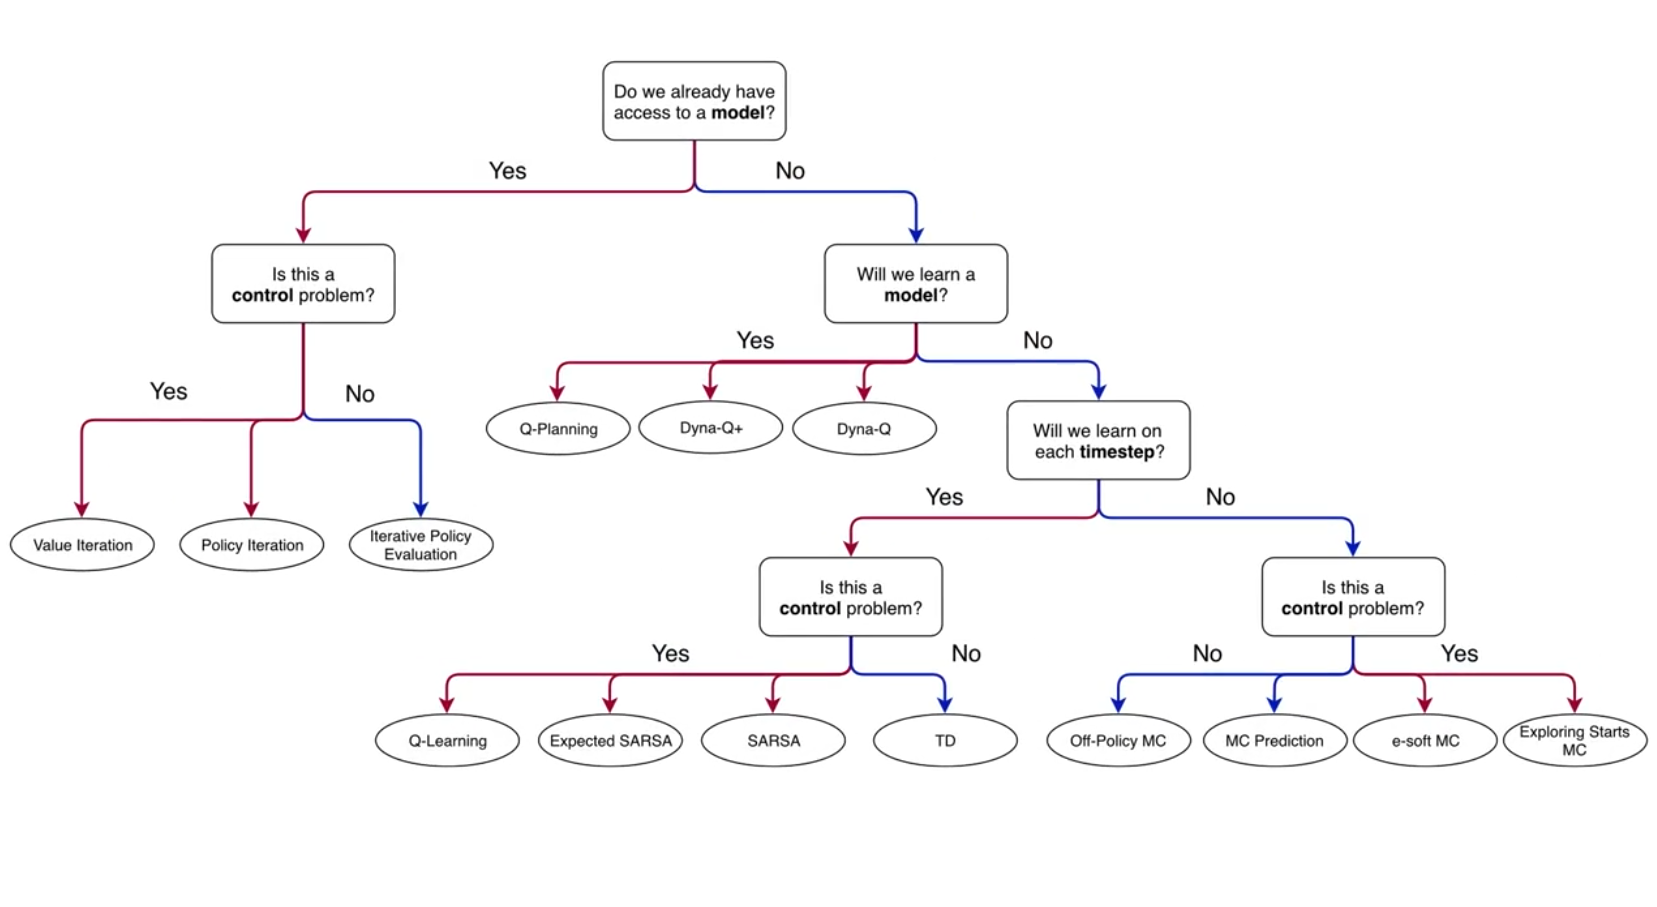
\includegraphics[scale = 0.3]{diagram_tabluar_methods.png}}
  \vspace{-7pt}
  \centerline{\footnotesize{(a)}}
\end{minipage}\\
\begin{minipage}[t]{1\linewidth}
  \centering
  \centerline{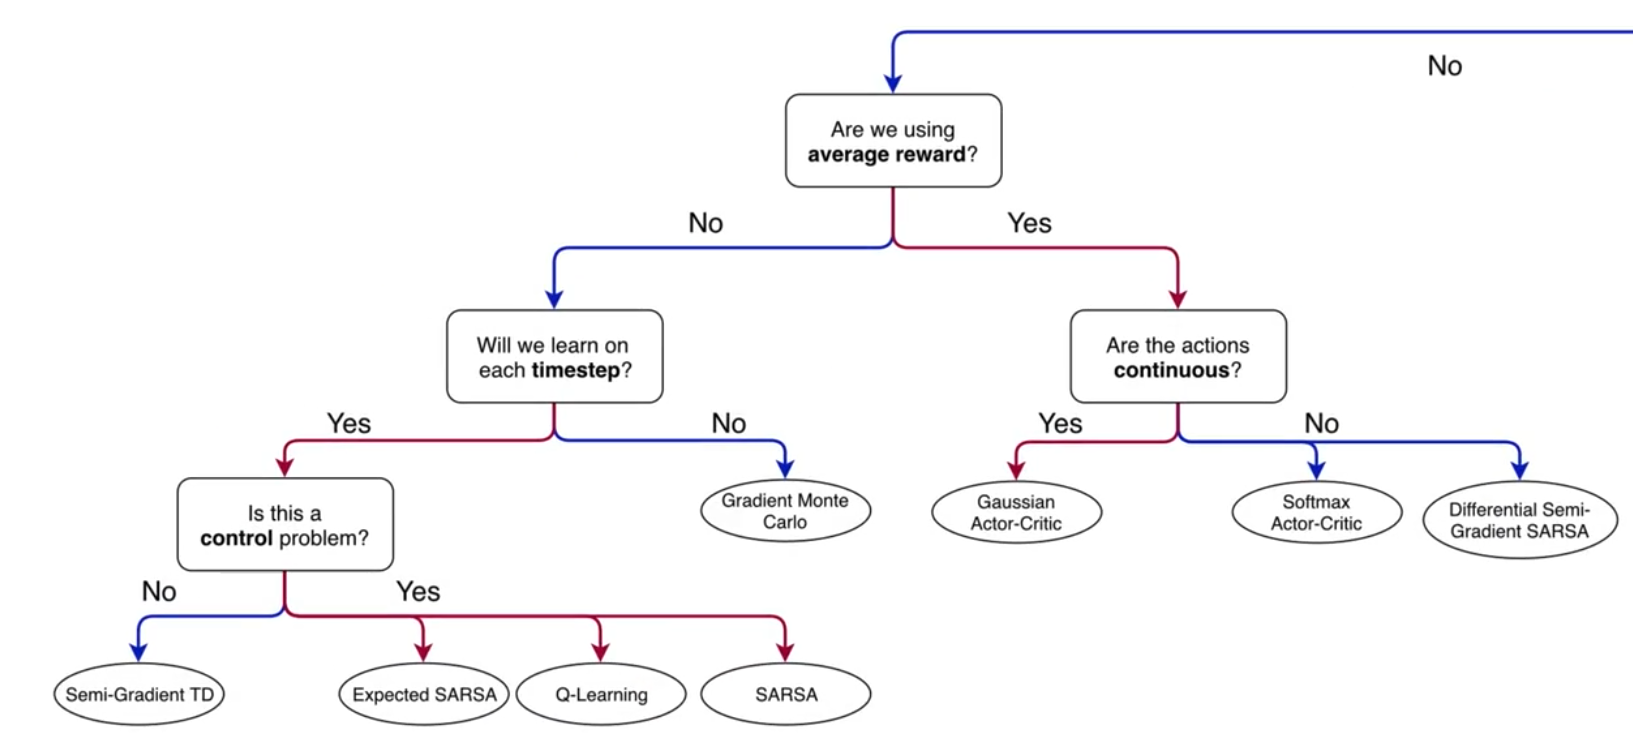
\includegraphics[scale = 0.3]{diagram_function_approximation_methods.png}}
  \vspace{-7pt}
  \centerline{\footnotesize{(b)}}
\end{minipage}
\caption{\footnotesize{\textbf{Tabular methods (a) and Function approximation methods (b) diagram}}}
\label{fig: diagram_tabluar_function_approximation_methods}
\end{figure}

The most important concepts in reinforcement learning is the \underline{\textbf{value function}}. A value function is a special \textbf{data structure} that \textbf{store} the \textbf{long-term gain} \underline{\textbf{locally}} and is \emph{accessible} at each time step of learning. Through value function, we formulate our problem into a series of \textbf{\underline{overlapping} \underline{subproblems} with \underline{common structure}}. At each timestep, given state/state-action pair, the \textbf{learning \underline{objective} of each subproblem} is defined using value function.  As the learning process continues, the \textbf{value function} will \textbf{approach to the ultimate learning goal} of our agents.  Therefore, an agent that exploit its policy choice over \textbf{local} estimate of value function is able to reach the \textbf{global optimal} policy in asympototic sense. With value function, we can design a recusive algorithm conveniently with linear time. 

Depending on how to represent the value function, the algorithms fall into two categories. See Figure \ref{fig: diagram_tabluar_function_approximation_methods} for a summary of all of these methods. 
\subsubsection{Tabular methods}
\textbf{Tabular methods}(lecture 4-7): The simplest way to represent and store the value function is via a table.  

A \textbf{tabular representation} of value function allows us to \textbf{maintain} and \textbf{update} the \emph{value} of each state or state-action pair \textbf{independently}. This type of presentation maximize the \textbf{discrimination} of the value function, but results in zero \textbf{generalization}. Generalization of value function means that updating value of one state would affect the value of other states. 

Tabular representation is suitable if $|\cS|$ and $|\cA|$ is relatively small. For many real world problem, a tabular representation for value of all actions and states are not feasible. 

We split our algorithm for tabular methods into algorithms for prediction and control: 
\begin{itemize}
\item \textbf{Control} (lecture 4): The policy improvement strategy is \underline{\textbf{fixed}}. According to \underline{\textbf{Policy}} \underline{\textbf{improvement}} \underline{\textbf{theorem}} for tabular methods, it is guaranteed that a greedy policy that maximize the action-value function is able to improve upon existing policy by increasing the value $v_{\pi}$. 
\begin{theorem} (\textbf{Policy improvement theorem})
Let $\pi$ and $\pi'$ be any pair of deterministic policies such that, for all $s \in \cS$, 
\begin{align}
q_{\pi}(s, \pi'(s)) &\ge v_{\pi}(s). \label{eqn: policy_improv_theorem_1}
\end{align}
Then the policy $\pi'$ must be\textbf{ as good as, or better than}, $\pi$. That is, it must obtain greater or equal expected return from all states $s \in \cS$:
\begin{align}
v_{\pi'}(s) &\ge v_{\pi}(s).  \label{eqn: policy_improv_theorem_2}
\end{align} Moreover, if there is strict inequality of \eqref{eqn: policy_improv_theorem_1} at any state, then there must be strict inequality of \eqref{eqn: policy_improv_theorem_2} at that state. 
\end{theorem}


\item \textbf{Prediction}(lecture 4-7): depending on our \textbf{knowledge} on the \textbf{environment}/\textbf{model}, we split again it into two classes of algorithms:
\begin{itemize}
\item \textbf{Model-based methods (Planning)} (lecture 4): when we have full access to model \emph{dynamic} $p(s', r|s, a)$ for all $s,a,r,s'$. In this case, we have \textbf{Bellman equation} and \textbf{Bellman optimality equation} (lecture 3) for $v_{\pi}, q_{\pi}, v_{*}, q_{*}$. The \textbf{dynamic programming (DP)} algorithm make \textbf{\emph{expected updates}} based on Bellman equation. 
\begin{align}
v_{\pi}(s) &=  \sum_{a}\pi(a|s)\sum_{s'}\sum_{r}p(s', r| s, a)\brac{r + \gamma v_{\pi}(s')}, \quad \forall\,\; s\in \cS \label{eqn: bellman_eqn_value} \\
&= \E{}{R_{t+1}  + \gamma\,v_{\pi}(S_{t+1}) | S_{t} = s} \label{eqn: bellman_eqn_value3}\\
q_{\pi}(s, a) &=\sum_{s', r}p(s', r|s,a)\brac{r+ \gamma \sum_{a'}\pi(a'|s')q_{\pi}(s', a')} \label{eqn: bellman_eqn_value_action}\\
&=\E{}{R_{t+1} + \gamma q_{\pi}(S_{t+1}, A_{t+1}) | S_{t}=s, A_{t}=a}  \label{eqn: bellman_eqn_value_action_3}
\end{align}
\begin{align}
v_{*}(s) &=  \max_{a\in \cA(s)}\E{}{R_{t+1} + \gamma v_{*}(S_{t+1}) | S_{t}=s, A_{t}=a} \label{eqn: bellman_eqn_optimal_value3}\\
&= \max_{a\in \cA(s)}\sum_{s'}\sum_{r}p(s', r|s, a)\brac{r + \gamma v_{*}(s')} \quad s\in \cS \label{eqn: bellman_eqn_optimal_value2} \\
q_{*}(s, a) &=  \E{}{R_{t+1} + \gamma \max_{a'\in \cA(s)}q_{*}(S_{t+1}, a') \Big| S_{t}=s, A_{t}=a} \label{eqn: bellman_eqn_optimal_value_action3}\\
&=\sum_{s'}\sum_{r}p(s', r|s, a)\brac{r + \gamma  \max_{a'\in \cA(s)}q_{*}(s', a')} \quad \forall\,\; s\in \cS, \; a\in \cA(s) \label{eqn: bellman_eqn_optimal_value_action2}
\end{align} There are \textbf{policy iteration methods} or \textbf{value iteration methods} based on whether or not we need to complete multiple \emph{sweeps} all states at each iteration or just one sweep of policy evaluation and one sweep for policy improvement, respectively. 

\item \textbf{Model-free methods (Learning)} (lecture 5-7): normally, the agent has little knowlege on the environment. The only way to learn is via \textbf{interation with environment}, i.e. at given observed state, generate a sample action and then collect sample rewards and observe sample next states. Compared to model-based learning method, model-free algorithms requires much less knowledge and much less resources. This is achieved at the expense of losing some efficiency via additional exploration  and accumulation.

The model-free algorithms is also called \textbf{sample-based methods}. It incrementally update the value function estimate using old estimate, and some \textbf{error term}. The error term is the main difference for these algorithms. For instance,
\begin{itemize}
\item  \textbf{Monte Carlo (MC) methods (lecture 5)} use directly the \textbf{sample return} in the error term. In order to obtain the sample return, one has to wait until the episode ends to update the value estimate and thus to update the policy. The advantage is that the value estimator from Monte Carlo methods is \textbf{unbiased} but with \textbf{high variance} and thus \textbf{slow learning}. MC methods can be applied to \textbf{off-policy} setting using \textbf{importance sampling}, where the ratio between target policy and behavior policy is used as importance weights.  The \emph{\textbf{sample updates}} for MC are
\begin{align*}
V(S_{t}) &\leftarrow V(S_{t}) + \alpha_{t}\paren{G_{t} - V(S_{t})} \\
Q(S_{t}, A_{t}) &\leftarrow Q(S_{t}, A_{t}) + \alpha_{t}\brac{G_{t}  - Q(S_{t}, A_{t})},
\end{align*} where $G_{t}$ is the sample return accumulated starting at $t+1$ until the end of episode.

\item  \textbf{Temporal Difference (TD) learning (lecture 6)} use \underline{\textbf{boostrapping}} to estimate the return based on the immediate reward plus the estimate of value at immediate next state. TD learning can update the value estimator at each time step, thus it is much \textbf{faster} in learning with much \textbf{lower variance}. On the other hand, it introduces additional \textbf{bias} since the target is affected by the quality of value estimator at its successor state.
\begin{align*}
V(S_{t}) &\leftarrow V(S_{t}) + \alpha_{t}\brac{\hat{G}_{t}  -  V(S_{t})}. \\
 \text{  \textbf{TD(0)} }\quad\hat{G}_{t} &= R_{t+1} + \gamma V(S_{t+1}).
\end{align*} For action-value function (control), the \emph{\textbf{sample updates}} are
\begin{align*}
Q(S_{t}, A_{t}) &\leftarrow Q(S_{t}, A_{t}) + \alpha_{t}\brac{\hat{G}_{t}  - Q(S_{t}, A_{t})}.  \\
 \text{  \textbf{Sarsa (on-policy)} }\quad\hat{G}_{t} &= R_{t+1} + \gamma Q(S_{t+1}, A_{t+1}) \\
\text{  \textbf{Q-Learning (off-policy)} }\quad\hat{G}_{t} &=  R_{t+1} + \gamma \max_{a'\in \cA(S_{t+1})}Q(S_{t+1}, a')  \\
 \text{  \textbf{Expected Sarsa (off-policy)} }\quad\hat{G}_{t} &= R_{t+1} + \gamma\sum_{a'}\pi(a'|S_{t+1})Q(S_{t+1}, a') .
\end{align*}
\end{itemize}
\end{itemize}
\end{itemize} 

\subsubsection{Function Approximation}

\textbf{Function approximation} (lecture 8-10): Tabular representation of value function or policy distribution is limited to small state space $|\cS|$ and small action space $|\cA|$. Base on the \textbf{curse of dimensionality}, as the dimension of state increases, the size of state space increases exponentially. For very large state space or action space, the only feasible solution is via function approximation. 

The performance of function approximation is measured via its ability for \textbf{generalization} and \textbf{discrimination}:
\begin{itemize}
\item  \textbf{\emph{Generalization}}, which means updating value of one state would affect the value of other states. That is, the change \emph{\underline{generalizes}} from that state to affect the values of many other states. Aggregate all states would easily achieve high generalization but with no discrimination. 

\item \textbf{\emph{Discriminization}}, which means the ability to make the value of two states different. If value of each states are represented independently, such as tabular methods, the discrimination is maximized but there is no generalization. 
\end{itemize}

Compared to tabular representation, function approximation \textbf{encodes} the \emph{value function} or the \emph{policy distribution} into a set of \textbf{parameters}, i.e.  $\hat{v}(s) \rightarrow \hat{v}(\mb{s}, \mb{w})$ or $\hat{q}(s, a) \rightarrow \hat{q}(\mb{s}, a, \mb{w})$. The \textbf{dimension of parameters} is much less than the size of table when values of all states/action-states are stored. It is thus an \textbf{efficient representation} compared to tables. \textbf{Tabular representation} can be seen as \textbf{linear approximation} of value function using \textbf{one-hot encoding}. 

On the other side, however, the loss of discrimination power would lead to the \textbf{loss of \underline{\emph{policy}} \underline{\emph{improvement theorem}}}. It is no longer true that if we change the policy to improve the discounted value of one state then we are guaranteed to have improved the overall policy in any useful sense. That is, we \textbf{no longer} have a \textbf{fixed strategy} to obtain optimal policy given the value function. The good news is that by using \textbf{parameterized policy distribution}, we can learn optimal policy based on \underline{\emph{\textbf{policy gradient theorem}}} using \textbf{policy gradient methods}.

This leads to the change in each step of the Generalized Policy Iteration.
\begin{itemize}
\item \textbf{Prediction} (lecture 8-9): Compared to Tabular methods, the prediction task is very \textbf{similar} for function approximation methods. The main difference is that we do not directly update the value at each state/state-action pair. Instead, we incrementally \textbf{updates the parameter} $\mb{w}$ or the value function. 

The task of prediction with \emph{function approximation} is essentially a \textbf{\emph{\underline{supervised learning}} problem}. Given $(S_{t}, A_{t}, \hat{G}_{t})$, the objective is to find parameterized function $q_{\mb{w}}: \cS \times \cA \rightarrow \bR$ that minimize the \textbf{mean squared value error} (VE). The \textbf{target} $\hat{G}_{t}$ could be the \emph{sample returns} (MC) or the \emph{TD target} (TD). The optimal paramter $\mb{w}_{*}$ can be found via online algorithms such as stochastic gradient desent or semi-gradient methods:
\begin{itemize}
\item \textbf{Gradient Monte Carlo algorithm} via \textbf{stochastic gradient descent (SGD)}: 
\begin{align}
\mb{w}_{t+1} &\leftarrow  \mb{w}_{t} + \alpha \brac{\hat{G}_{t} - \hat{v}(S_{t}, \mb{w}_{t})} \grad{\mb{w}}{\hat{v}(S_{t}, \mb{w}_{t})} \label{eqn: sgd_fun_approx} \\
\mb{w}_{t+1} &\leftarrow  \mb{w}_{t} + \alpha \brac{\hat{G}_{t} - \hat{q}(S_{t}, A_{t}, \mb{w}_{t})} \grad{\mb{w}}{\hat{q}(S_{t},  A_{t}, \mb{w}_{t})} \nonumber
\end{align} where $\hat{G}_{t} = G_{t}$ is the sample return obtained at end of each episodes. 

\item \textbf{Temporal difference learning} via \textbf{semi-gradient methods}:
\begin{align}
\mb{w}_{t+1} &\leftarrow  \mb{w}_{t} + \alpha \delta_{t}\grad{\mb{w}}{\hat{v}(S_{t}, \mb{w}_{t})} \label{eqn: td_fun_approx}
\end{align} where $\delta_{t} = R_{t+1} + \gamma \hat{v}(S_{t+1}, \mb{w}_{t}) - \hat{v}(S_{t}, \mb{w}_{t})$ is the \textbf{TD error}.
\end{itemize} For action-value function, we have
\begin{align}
\mb{w}_{t+1} &\leftarrow  \mb{w}_{t} + \alpha\, \delta_{t}\,\grad{\mb{w}}{\hat{q}(S_{t}, A_{t}, \mb{w}_{t})}  \nonumber\\
\text{  \textbf{SARSA} }\quad \delta_{t} &= \brac{R_{t+1} + \gamma \hat{q}(S_{t+1}, A_{t+1}, \mb{w}_{t}) - \hat{q}(S_{t}, A_{t}, \mb{w}_{t})} \label{eqm: semi_grad_sarsa}\\
\text{  \textbf{Q-Learning} }\quad \delta_{t}&:=\brac{R_{t+1} + \gamma \max_{a'}\hat{q}(S_{t+1}, a', \mb{w}_{t}) - \hat{q}(S_{t}, A_{t}, \mb{w}_{t})}   \label{eqn: semi_grad_q_learning}\\
 \text{  \textbf{Expected Sarsa} }\quad \delta_{t} &= \brac{R_{t+1} +\gamma\sum_{a'}\pi(a'|S_{t+1})\hat{q}(S_{t+1}, a', \mb{w}_{t}) - \hat{q}(S_{t}, A_{t}, \mb{w}_{t})}  \label{eqn: semi_grad_exp_sarsa} 
\end{align} 

Note that the problem we are solving in policy evalution/prediction has violated many \textbf{assumptions} in supervised learning:
\begin{itemize}
\item While the supervised learning assume the samples are \textbf{\emph{independent}} \emph{identically distributed}, this is \textbf{not true} for policy evalution task with function approximation. Since successive states $(S_{t}, A_{t}, G_{t})_{t \ge \tau}$ follows a MDP, which are naturally correlated. 

\item Most supervised learning methods are not designed for \textbf{online learning} setting, while the reinforcement learning required online learning ability as rewards are obtained sequentially. 

\item By using \textbf{boostrapping} in the \textbf{target} like TD learning, we make the target depend on the approximated function evaluted at successor state. This introduce additonal \textbf{bias} as well as the \emph{\textbf{positive feedback loop}} caused by the \textbf{error} of value function approximation as well as \textbf{asympototic dependencies}.  This makes the target function dynamic and changing during the learning process. 
\end{itemize}
Since the assumption of supervised learning methods are violated, many theoretical \textbf{convergence guarantees do not hold}. In fact, with boostrapping in target, many complex models such as neural networks are likely to \textbf{diverge}. This is especially true in off-policy learning such as Q-learning, which is called \textbf{Off-policy Divergence}.

We also learned two special classes of function approximation: \textbf{linear methods} and \textbf{artificial neural network}.
\begin{itemize}
\item \textbf{Linear methods} is the simplest function approximation. The key is to design a good feature mapping for state. 
\begin{align}
\hat{v}(s, \mb{w}_{t}) &= \sum_{k}w_{k,t} \phi_{k}(s) = \inn{ \mb{w}_{t}}{\mb{\phi}(s)} \label{eqn: generalized_linear_form}
\end{align} where $\mb{\phi}$ is the \textbf{feature mapping}. Popular choice of feature mapping functions includes \textbf{functional basis} such as Fourier Basis, RBF, RKHS. We also generalize the one-hot encoding to have \textbf{coarse coding}, \textbf{tile coding} etc.

\item \textbf{Artificial neural network (ANN)}. \textbf{Deep learning architectures} vary a lot for different  applications and state definition. For instance, if the state is image, then Convolutional Neural Network (CNN) is preferred. Deep learning can be applied to Q-learning to have the \textbf{\emph{Deep Q-Network (DQN)}} \citep{franccois2018introduction}  algorithm. Check other deep RL models in \citep{franccois2018introduction}

ANN is highly \textbf{non-linear}, \textbf{non-convex} model, which makes it very \emph{sensitive} to the change of target. Thus, boostrapping in target is very likely to cause the learning algorithm diverge. 
\end{itemize}

\item \textbf{Control} (lecture 10): As discussed above, policy improvement theorem does not hold for function approximation. However, by using \textbf{parameterized policy distribution} $\pi \rightarrow \pi(a|\mb{s}, \mb{\theta})$, we can find another way to find optimal policy: \underline{\textbf{policy gradient method}}. 

In fact, we have the \underline{\textbf{policy gradient theorem}} which  gives an exact formula for how performance is affected by the policy parameter that does not involve \underline{derivatives} of \underline{the state distribution}. Like how policy improvement theorem leads to a fixed strategy in Tabular methods, this policy gradient theorem provides a theoretical foundation for all policy gradient methods.
\begin{theorem} (\textbf{Policy gradient theorem})
For both the episodic case and continuing case under ergodic MDP, the objective functions $\cR(\mb{\theta})$ are defined as in \eqref{eqn: obj_policy_grad_episodic} and \eqref{eqn: obj_policy_grad_continuing} respectively. Then 
\begin{align}
\grad{\mb{\theta}}{\cR(\mb{\theta})} &\propto \sum_{s}\mu_{\pi(\mb{\theta})}(s)\sum_{a}\grad{\mb{\theta}}{\pi(a |\mb{s}, \mb{\theta})}q_{\pi}(\mb{s}, a) \label{eqn: policy_grad_theorem}\\
&= \E{\mb{s} \sim \mb{\mu}_{\pi(\mb{\theta})}}{\sum_{a}\grad{\mb{\theta}}{\pi(a |\mb{s}, \mb{\theta})}q_{\pi}(\mb{s}, a) } \label{eqn: policy_grad_theorem2} \\
&= \E{\mb{s} \sim \mb{\mu}_{\pi(\mb{\theta})}}{\E{a \sim \pi(a|\mb{s}, \mb{\theta})}{\grad{\mb{\theta}}{\log \pi(a |\mb{s}, \mb{\theta})}q_{\pi}(\mb{s}, a) }},\label{eqn: policy_grad_theorem3}
\end{align} where $\mb{\mu}_{\pi}$ is the limiting state distribution under $\pi$, $\mu(s) = \lim_{t\rightarrow \infty}Pr\{S_{t} = s| S_{0}, \pi\}$, (or on-policy distribution under policy $\pi$).  In particular, the gradient of objective does not depend on the gradient of state distribution $\grad{}{\mb{\mu}}$.  For ergodic MDP with average reward objective, the equation \eqref{eqn: policy_grad_theorem} is exact. For episodic task, the constant of proportionality is the average length of an episode.
\end{theorem}

We have the following \textbf{policy gradient methods}:
\begin{itemize}
\item \textbf{REINFORCE} (\textbf{stochastic gradient ascent} with \textbf{Monte Carlo} methods):
\begin{align}
\mb{\theta}_{t+1} &\leftarrow \mb{\theta}_{t} + \alpha \;G_{t}\grad{\mb{\theta}}{\log\pi(A_{t}|S_{t}, \mb{\theta})}, \label{eqn: reinforce_update}
\end{align} where $G_{t}$ is the sample return obtained at the end of each episode. 

\item \textbf{REINFORCE} with \textbf{baseline}: adding baseline function (function of state) helps to reduce variance in REINFORCE
\begin{align}
\mb{\theta}_{t+1} &\leftarrow \mb{\theta}_{t} + \alpha \;(G_{t}-\hat{v}(S_t, \mb{w}_t))\grad{\mb{\theta}}{\log\pi(A_{t}|S_{t}, \mb{\theta})}, \label{eqn: reinforce_update_w_baseline}
\end{align} and the weight for value function is updated using Gradient Monte Carlo method \eqref{eqn: sgd_fun_approx}. 

\begin{figure}
\begin{minipage}[t]{1\linewidth}
  \centering
  \centerline{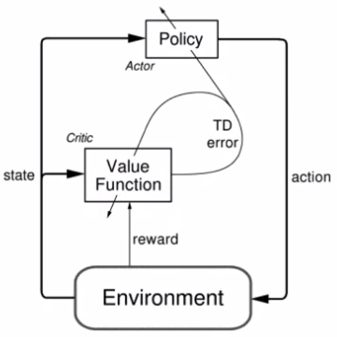
\includegraphics[scale = 0.5]{actor_critic.png}}
\end{minipage}
\caption{\footnotesize{\textbf{The Actor-Critic methods}}}
\label{fig: actor_critic}
\end{figure}
\item \textbf{Actor-Critic methods}: See Figure \ref{fig: actor_critic}. In actor-critic methods, both value estimation and policy optimization is done iteratively based on \textbf{TD error}. The actor produce optimal policy given value and the critic evalute the policy by updating the value, then the actor optimize the policy based on new value.
\begin{itemize}
\item \textbf{Actor}: the role of an \textbf{actor} is to \textbf{\emph{update the policy distribution}} via policy gradient algorithm.  The updates for \emph{actor} is shown below
\begin{align}
\mb{\theta}_{t+1} &\leftarrow \mb{\theta}_{t} + \alpha_{\mb{\theta}}  \;\underline{\delta_t}\; \grad{\mb{\theta}}{\log\pi(A_{t}|S_{t}, \mb{\theta})} \label{eqn: actor_update}
\end{align} where 
\begin{align*}
\delta_{t}&= R_{t+1} + \gamma \hat{v}(S_{t+1}, \mb{w}_{t}) - \hat{v}(S_{t}, \mb{w}_{t})
\end{align*}
 is the \textbf{TD error}. The update in \textbf{actor} is to \textbf{increase} the \textbf{value function} under new policy.

\item \textbf{Critic}: Given the learned policy $\pi(a|\mb{s}, \mb{\theta})$, the role of a \textbf{critic} is to \textbf{\emph{evalute and update} the \emph{value} of the policy} and used it as a \textbf{feedback} for actor's performance. As shown in Figure \ref{fig: actor_critic}, the same TD error $\delta_t$ is used by \textbf{semi-gradient methods} (e.g. TD(0)) for function apprximation.
\begin{align}
\mb{w}_{t+1} &\leftarrow  \mb{w}_{t} + \alpha_{\mb{w}} \;\underline{\delta_{t}}\; \grad{\mb{w}}{\hat{v}(S_{t}, \mb{w}_{t})}  \label{eqn: critic_update}
\end{align} The updates in \textbf{critics} is to adjust the value function to \textbf{match} the target value.
\end{itemize}

There are several commonly used parameterized policy distribution:
\begin{itemize}
\item  When $\cA$ is \textbf{finite discrete}, and $\mb{s} \in \cS$, we can ues the \textbf{soft-max function} to approximate the policy function
\begin{align}
\pi(a |\mb{s}, \mb{\theta}) &= \frac{\exp\paren{h(\mb{s}, a, \mb{\theta})}}{\sum_{a'}\exp\paren{h(\mb{s}, a', \mb{\theta})}} \label{eqn: soft_max_policy} \\
\log \pi(a |\mb{s}, \mb{\theta}) &= h(\mb{s}, a, \mb{\theta}) -  \underline{\log \sum_{a'}\exp\paren{h(\mb{s}, a', \mb{\theta})}}  \label{eqn: log_soft_max_policy} \\
\grad{\mb{\theta}}{\log \pi(a |\mb{s}, \mb{\theta}) } &= \grad{\mb{\theta}}{h(\mb{s}, a, \mb{\theta})} - \underline{\E{\pi(a |\mb{s}, \mb{\theta}) }{ \grad{\mb{\theta}}{h(\mb{s}, a, \mb{\theta})}}}   \label{eqn: grad_log_soft_max_policy} \\
&= \grad{\mb{\theta}}{h(\mb{s}, a, \mb{\theta})} - \sum_{a'}\pi(a' |\mb{s}, \mb{\theta}) \grad{\mb{\theta}}{h(\mb{s}, a', \mb{\theta})} \nonumber
\end{align}

\item When $\cA \subset \bR^{k}$ is \textbf{continuous space},  and $\mb{s} \in \cS$, $\mb{\theta} = [\mb{\theta}_{\mu}, \mb{\theta}_{\sigma}]$
\begin{align}
\pi(a |\mb{s}, \mb{\theta}) &= \frac{1}{\sqrt{2\pi}\sigma(\mb{s}, \mb{\theta}_{\sigma})}\exp\paren{-\frac{(a - \mu(\mb{s}, \mb{\theta}_{\mu}))^2}{2\sigma(\mb{s}, \mb{\theta}_{\sigma})^2}}
 \label{eqn: normal_policy}
\end{align} where 
\begin{align*}
\mu(\mb{s}, \mb{\theta}_{\mu}) &= \inn{\mb{\theta}_{\mu}}{\mb{\phi}_{\mu}(\mb{s})} \\
\sigma(\mb{s}, \mb{\theta}_{\sigma}) &= \exp(\inn{\mb{\theta}_{\sigma}}{\mb{\phi}_{\sigma}(\mb{s})})
\end{align*} Note that
\begin{align*}
\grad{\mb{\theta}_{\mu}}{\log \pi(a |\mb{s}, \mb{\theta}) } &= \frac{1}{\sigma(\mb{s}, \mb{\theta}_{\sigma})^2}\paren{a - \mu(\mb{s}, \mb{\theta}_{\mu})}\mb{\phi}_{\mu}(\mb{s}) \\
\grad{\mb{\theta}_{\sigma}}{\log \pi(a |\mb{s}, \mb{\theta}) }&= \paren{\frac{(a - \mu(\mb{s}, \mb{\theta}_{\mu}))^2}{\sigma(\mb{s}, \mb{\theta}_{\sigma})^2} - 1}\mb{\phi}_{\sigma}(\mb{s})
\end{align*}
\end{itemize}

\end{itemize}

\end{itemize}



\subsection{Learning vs. Planning}
In many situation, we may not have \emph{full} information on our environment, but we have \emph{some} knowledge of it. This knowledge is maintained via a model. A \emph{\textbf{model}} of the environment means anything that an agent can use to predict how the environment will respond to its actions. Given a state and an action, a model \textbf{produces} a prediction of the resultant next state and next reward. A model is the \textbf{inner world} of an agent, which should \textbf{match the real world} during the learning process. Planning is \textbf{preferred} when
\begin{itemize}
\item there lacks of \textbf{immediate} \textbf{frequent} \textbf{feedbacks} from the real world. Many environments produce \emph{\textbf{sparse}} and \textbf{\emph{delayed}} rewards, which prohibits agents to explore and exploit efficiently.
\item the \textbf{cost} of interacting with environment and obtaining real experience is \textbf{expensive}. For example, car crushing experiments, or flight pilot training program. The cost of a failure is not recovered. 
\item the \textbf{size} of training data is limited. This is similar to the situtation when the generative model is preferred over discriminative model in supervised learning.
\item there exists \textbf{good model} that closely \textbf{match} the real world experience. Typical example is \textbf{games} or the classical \textbf{physical} \textbf{experiments}, where the dynamic can be precisely modeled. 
\end{itemize} Unlike the environment that generates the  \underline{\emph{\textbf{real} experience}}, a model is used to \underline{\emph{\textbf{simulate}}} the environment and produce \underline{\emph{\textbf{simulated experience}}}. The task of agent  (lecture 7) is to learn from interaction with both real experience (i.e. \textbf{direct RL}) as well as simulated experience (i.e. \textbf{indirect RL}) while maintaining and learning the model (i.e. \textbf{model learning}). The \textbf{planning} is the process of learning from simulated experience. Figure \ref{fig: Planning_learning_relationship} shows how the \textbf{learning and planning are integrated} in the agent's system. 
\begin{figure}
\begin{minipage}[t]{1\linewidth}
  \centering
  \centerline{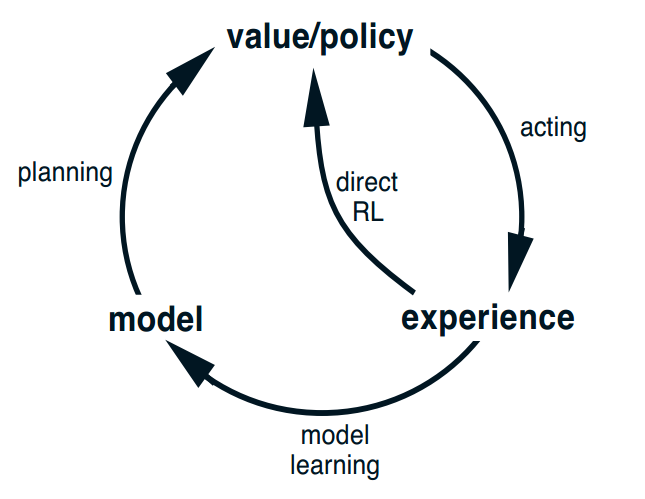
\includegraphics[scale = 0.3]{Planning_learning_relationship.png}}
\end{minipage}
\caption{\footnotesize{\textbf{The generic relationship between model learning, direct RL, planning in a planning agent. Note that the value/policy can be updated either by real experience via direct RL or by simulated experience via planning. Meanwhile, the real experience will be used for model update/learning. }}}
\label{fig: Planning_learning_relationship}
\end{figure}
There are two type of models:
\begin{itemize}
\item \emph{\textbf{distribution models}}: models produce a description of \emph{all possible} next-state-reward pairs and their probabilities, i.e. $p(s', r| s, a)$ for all next-state-reward pairs $s', r$ given every state $s$ and action $a$. Distribution models are \emph{stronger} than sample models in that they can always be used to produce samples. A useful class of distribution models is the \textbf{\emph{Probabilistic Graphical Model}} \citep{koller2009probabilistic} including the \emph{Bayesian Networks}, \emph{Markov Networks}, \emph{Gaussian  Graphical Models}, etc. These models use graph representation to \emph{factorize} the global joint distribution between states, actions and rewards into several connected local factors embedded in subgraphs. 

\item \emph{\textbf{sample models}}:  models produce just one of the possibilities, \emph{sampled} according to the probabilities. Given probabilistic models, one can use \textbf{sampling methods} \citep{liu2001monte} such as \emph{Importance Sampling},  \emph{sequential sampling} such as \emph{Gibs sampling}, \emph{Markov Chain Monte Carlo (MCMC)}, or \emph{Gradient Flow methods} etc to obtains samples of actions and states. 
\end{itemize}

Within a planning agent, there are at least two roles for \textbf{real experience}: 
\begin{itemize}
\item \textbf{\emph{\underline{model learning}}}: i.e.   \textbf{improve the model} to make it more accurately \emph{match} the real environment;
\item \textbf{\emph{\underline{direct reinforcement learning (direct RL)}}}: i.e. directly \textbf{improve the value function} and \textbf{policy} using the kinds of reinforcement learning methods. All RL methods discussed before can be used here. 
\end{itemize} 
Figure \ref{fig: Planning_learning_relationship} describes the major components in a planning agent and their interactions.  Note how experience can improve value functions and policies either \emph{directly} or \emph{indirectly} via the model. It is the latter, which is sometimes called \textbf{\emph{\underline{indirect} reinforcement learning}} (i.e. learn via simulated experience), that is involved in \underline{\emph{\textbf{planning}}}.

\begin{figure}
\begin{minipage}[t]{1\linewidth}
  \centering
  \centerline{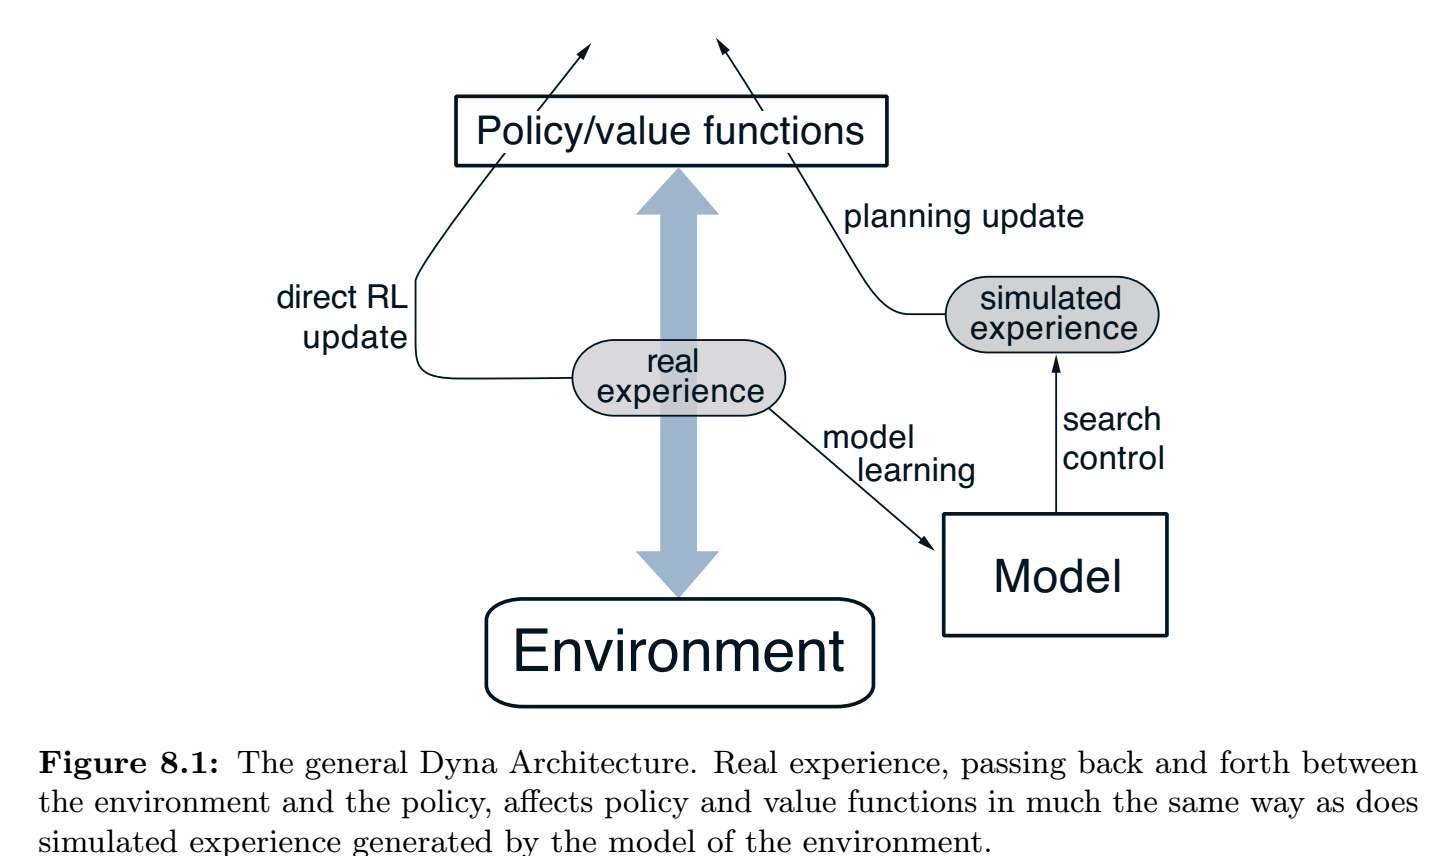
\includegraphics[scale = 0.3]{Dyna_Q.png}}
\end{minipage}
\caption{\footnotesize{\textbf{The Dyna-Q architecture. }}}
\label{fig: Dyna_Q}
\end{figure}
Figure \ref{fig: Dyna_Q} shows the architecture in \textbf{\emph{Dyna-Q}},  an architecture integrating the major functions needed in an \emph{online planning agent}.  It has the following components:
\begin{itemize}
\item \textbf{planning}:  use  random-sample one-step tabular Q-planning method. 
\item \textbf{direct RL}:  one-step tabular Q-learning discussed in last chapter. Typically, as in Dyna-Q, the \emph{same} reinforcement learning method is used both for learning from real experience and for planning from simulated experience. The reinforcement learning method is thus the "\emph{final \textbf{common path}}" for both learning and planning.
\item \textbf{model-learning}: \textbf{\emph{table-based}} and assumes the environment is \textbf{\emph{deterministic}}, i.e. given state-action pair, the output of model is \textbf{fixed} reward and next-state pair. It can be coded as \emph{dictionary of dictionaries}. Under this assumption, model learning is simply saving the next state $S_{t+1}$ and reward $R_{t+1}$ for each experienced state $S_{t}$ and action $A_{t}$.
\item \textbf{\emph{search control}}:  the process that selects the \textbf{starting states} and \textbf{actions} for the simulated experiences generated by the model. 

\end{itemize} 

\subsection{Reward and Average reward}
\begin{itemize}
\item \textbf{Returns for episodic task} (lecture 3): In episodic task, the task is terminated at some time $T$. The return is a finite number
\begin{align}
G_{t} &= \sum_{\tau=0}^{T-t-1}R_{\tau+t+1} < \infty \label{eqn: returns_episodic}
\end{align}

\item \textbf{Discounted returns for continuing task} (lecture 3): In continuing task, there is no termination and the natural sum is infinite thus improper. In order to obtain finite return, we need to add discount factor $\gamma \in [0, 1)$
\begin{align}
G_{t} &= \sum_{\tau=0}^{\infty}\gamma^{\tau} R_{\tau+t+1} < \infty \label{eqn: returns_discount_continuing}
\end{align} Note that the choice of $\gamma$ has significant impact on the behavior of learning agents. When $\gamma \rightarrow 1$, the agent emphasize the long-term gain over shot-term gain. When $\gamma \rightarrow 0$, it does the opposite.  

Unlike the tabular cases, in which the returns from each state can be separately identified and averaged, using the discounted returns for function approximation in counting tasks is \textbf{questionable}, esp. when the MDP is ergodic and has become \textbf{stationary} in the long run.  In \textbf{ergodic continuing task}, because all states are the same, thus the \emph{average} of the returns will be the asympototic discount factor $\frac{1}{1-\gamma}$ times the \textbf{average reward}, or $r(\pi)/(1-\gamma)$.  


\item \textbf{Average reward for ergodic continuing task} (lecture 9): If a MDP is ergodic, i.e. $$\mu_{\pi}(s) = \lim_{t\rightarrow \infty} \text{Pr}\{S_t =s |A_{0:t-1} \sim \pi\},$$ which is assumed to exist for any $\pi$ and to be \textbf{independent} of $S_0$, the state distribution $\mu_{\pi}(s)$ does not change over time. At this status, the return defined as the cumulative reward function above is \emph{meaningless}, since at time $t$ and at time $t+1$ the underling system has not changed stochastically. Instead, we just need to consider the average-reward. In the average-reward setting, the quality of a policy $\pi$ is defined as the \emph{\textbf{average rate} of \textbf{reward}}, or simply \textbf{average reward}, while following that policy, which we denote as $r(\pi)$:
\begin{align}
r(\pi) &= \lim_{T\rightarrow \infty}\frac{1}{T}\E{\pi}{G_{0:T} \big| S_{0}, A_{0:t-1} \sim \pi} \nonumber\\
 &=\lim_{T\rightarrow \infty}\frac{1}{T}\sum_{t=0}^{T}\E{\pi}{R_{t} \big| S_{0}, A_{0:t-1} \sim \pi}  \label{eqn: avg_reward_discount_continuing}\\
&= \lim_{t\rightarrow \infty}\E{\pi}{R_{t} \big| S_{0}, A_{0:t-1} \sim \pi}  \label{eqn: avg_reward_discount_continuing2}\\
&= \sum_{s}\mu_{\pi}(s)\sum_{a}\pi(a|s) \sum_{s', r}p(s', r| s, a)r,  \label{eqn: avg_reward_discount_continuing3}
\end{align}  where the expectations are conditioned on the initial state, $S_0$, and on the subsequent actions, $A_0, A_1, \ldots, A_{t-1}$, being taken according to $\pi$. $\mu_{\pi}(s)$ is the \underline{\textbf{steady-state distribution}}. We consider $\pi_{*} = \argmax_{\pi}r(\pi)$ as the \textbf{optimal policy}, which is the basis for \textbf{policy-based learning} algorithm. 

Moreover, according to MDP, the stationary distribution is the \textbf{fixed-point solution} the equation below:
\begin{align}
\mu_{\pi}(s') &= \sum_{s}\mu_{\pi}(s)\paren{\sum_{a}\pi(a|s) \sum_{s'}p(s'| s, a)} \label{eqn: stationary_dist_eqn}
\end{align} 

With the average rewards, we can define the the \textbf{differential return} as the cumulative \emph{difference} between rewards and the average reward:
\begin{align}
G_{t} &= \sum_{\tau=0}^{\infty}\paren{R_{\tau+t+1} - r(\pi)} < \infty \label{eqn: returns_diff_continuing}
\end{align}  Replacing \eqref{eqn: returns_discount_continuing} or \eqref{eqn: returns_episodic} with \eqref{eqn: returns_diff_continuing}, we can obtain the definition of \textbf{\emph{differential value function}} of expected differential returns given state or state-action pair: $v_{\pi}(s):= \E{\pi}{G_{t}  | S_{t}=s}$ and $q_{\pi}(s, a):= \E{\pi}{G_{t}  | S_{t}=s, A_{t}=a}$.  The differential returns measures how well our policy behaves as compared to the average reward under a \textbf{fixed policy}. We can also reformulate the \textbf{Bellman equation} and \textbf{Bellman optimality equation} for \textbf{average reward MDP} by removing $\gamma$ and replacing reward $r$ with differential reward $r-r(\pi)$.
\begin{align}
v_{\pi}(s) &= \sum_{a}\pi(a|s)\sum_{s', r}p(s', r| s, a)\brac{r - r(\pi) + v_{\pi}(s')}, \quad \forall\,\; s\in \cS \label{eqn: bellman_eqn_value_diff} \\
&= \E{\pi}{R_{t+1} - r(\pi)  + \,v_{\pi}(S_{t+1}) | S_{t} = s} \label{eqn: bellman_eqn_value_diff_2}\\
q_{\pi}(s, a) &=\sum_{s', r}p(s', r|s,a)\brac{r - r(\pi) +  \sum_{a'}\pi(a'|s')q_{\pi}(s', a')} \quad \forall\,\; s\in \cS, \; a\in \cA(s) \label{eqn: bellman_eqn_value_action_diff}\\
&=\E{\pi}{R_{t+1} - r(\pi)  + q_{\pi}(S_{t+1}, A_{t+1}) | S_{t}=s, A_{t}=a}  \label{eqn: bellman_eqn_value_action_diff_2}\\
v_{*}(s) &= \max_{a\in \cA(s)}\sum_{s', r}p(s', r|s, a)\brac{r - \max_{\pi}r(\pi) + v_{*}(s')} \label{eqn: bellman_opt_eqn_value_diff}\\
 &=  \max_{a\in \cA(s)}\E{}{R_{t+1} - \max_{\pi}r(\pi) + v_{*}(S_{t+1}) | S_{t}=s, A_{t}=a} \label{eqn: bellman_opt_eqn_value_diff_2} \\
 q_{*}(s, a) &=\sum_{s'}\sum_{r}p(s', r|s, a)\brac{r  - \max_{\pi}r(\pi) +  \max_{a'\in \cA(s)}q_{*}(s', a')}  \label{eqn: bellman_opt_eqn_value_action_diff}\\
 &=  \E{}{R_{t+1}  - \max_{\pi}r(\pi)+ \max_{a'\in \cA(s)}q_{*}(S_{t+1}, a') \Big| S_{t}=s, A_{t}=a} \label{eqn: bellman_opt_eqn_value_action_diff_2}
\end{align}
\end{itemize}


\newpage
\bibliographystyle{plainnat}
\bibliography{reference.bib}
\end{document}